Таким образом, мы определили структуру нашего проекта. Схематично она отражена на рис.~\ref{package_diagram_main}. Всего мы выделили четыре модуля:

\begin{itemize}
\item \texttt{Development} "--- библиотека для разработки задач;
\item \texttt{Testing} "--- ядро тестирующей системы;
\item \texttt{FileSystem} "--- работа с файлами;
\item \texttt{Interaction} "--- взаимодействие с пользоваталем.
\end{itemize}

\begin{figure}[h]
\center{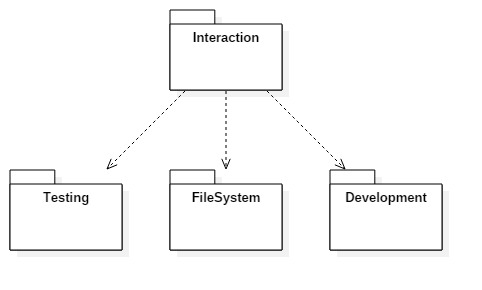
\includegraphics[scale=0.8]{package_diagram_main}}
\caption{Структура проекта}
\label{package_diagram_main}
\end{figure}

Как можно видеть на диаграмме, модули связаны между собой зависимостями. Эти зависимости подразумевают собой обычное использование классов из другого модуля, то есть никакая инъекция зависимостей здесь не используется. Хотя идея о её использовании рассматривалась, было принято решение от неё отказаться, так как инъекция зависимостей не приносила особых преимуществ.

Каждый из модулей \texttt{Development}, \texttt{Testing} и \texttt{FileSystem} "--- полностью независим от всех остальных. Это означает, что любой из них можно безболезненно отделить от всего проекта и свободно использовать где-то ещё, как самостоятельную библиотеку простых Java-классов.

Впрочем, такой подход порождает ряд сложностей, поскольку, к примеру, модуль тестирования не может напрямую обращаться к методам доступа из модуля файловой системы, хотя должен производить непосредственную манипуляцию файлами. По той же причине в модуле со средствами разработки отсутствует возможность компилировать код, потому что код для компиляции находится в модуле тестирования.

Однако все эти проблемы легко решаются посредством введения интерфейсов-посредников. В модуле взаимодействия с пользователем, выступающим связующим звеном между остальными модулями, эти интерфейсы реализуются так, как того требует ситуация, и здесь уже не возникает проблем, потому что есть доступ к коду любого модуля.